\documentclass[./main.tex]{subfiles}
\graphicspath{{\subfix{./Abbildungen/}}}

\begin{document}
\renewcommand{\tasktitle}{Titel$^1$}
\renewcommand{\taskpoints}{30} %Gesamtpunktzahl der Aufgabe
\renewcommand{\taskweight}{17}
\aufgabenanfang% Beginn der Aufgabe
\footnotetext[1]{Test}

Dies ist ein Template zur Erstellung und Formatierung von IChO-Aufgaben (Klausurrunden 2–4) und Cds-Aufgaben in \LaTeX. 
Dies ist ein Beispiel f\"ur einen Einleitungstext zu einer Aufgabe. Es gibt zudem die Option diesen Text in einen Kasten zu setzen wie es ja bei der internationalen Runde \"ublich ist.\\
\textit{F\"ur kursive Hervorhebung kann dies genutzt werden}. \textbf{F\"ur fette Hervorhebung dies}.

\teilaufgabe{In diesem Bereich steht eine Teilaufgabe}{Hier kann ein Hinweis hinzugef\"ugt werden}
\kasten{2.5cm}{
    Hiermit l\"asst sich ein Kasten erstellen zur Bearbeitung der Aufgabe.
    Die L\"ange des Kastens wird im Ersten Argument angegeben.
    L\"osungsk\"astchen folgen jeweils direkt auf die Aufgabenstellung – es gibt seit einigen Jahren keine Antwortb\"ogen mehr!
    Musterl\"osung bzw Bewertungshinweise werden mit dem Command \textbackslash kommentar \{Hier direkt notiert\}:\\ %Zeilenumbruch
    \kommentar{Dies ist eine Musterl\"osung}\punkte{1}
}{Nur dieser Text erscheint in der Sch\"ulerversion}

Die folgenden Abschnitte enthalten einige Beispiel-Teilaufgaben. Die Aufgabenteile b) und c) dienen als Beispiele f\"ur Multiple-Choice-Aufgaben. 
\teilaufgabe{\operator{Kreuze an} welche Antwortm\"oglichkeiten hier richtig sind.}{Die Reihenfolge der richtigen Antworten wir in dem \textbackslash MC Command im 6.ten Argument mit einer Zeichenkette bspw.: oxoox, ausgedr\"uckt die f\"ur die richtigen Antworten je ein x notiert}
Vor dem MC command folgt mit \textbackslash punkte wieder die Punktzahl\punkte{2}\par
\MC{A}{B}{C}{D}{E}{oxoox}
Bevorzugt wird eine richtig/falsch Auswahl, da hier ein falsch Ankreuzen auch bepunktet werden kann.\par % falls vor einem MC-Kasten noch Text stehen soll, muss an diesen ein \par angef\"ugt werden!
\MCrf{A}{B}{C}{D}{E}{oxoox}
\teilaufgabe{\operator{Kreuze an} welche Antwortm\"oglichekeiten hier richtig sind.\punkte{1}}{}
\MCvAnfang
\MCv{x}{Eine richtige L\"osung}
\MCv{o}{Eine falsche L\"osung}
\MCv{o}{Eine falsche L\"osung}
\MCv{o}{Eine falsche L\"osung}
\MCv{o}{Eine falsche L\"osung}
\MCv{o}{Eine falsche L\"osung}
\MCvEnde

Auch hier mit richtig/falsch m\"oglich:\par
\MCvrfAnfang
\MCv{x}{Eine richtige L\"osung}
\MCv{o}{Eine falsche L\"osung}
\MCv{o}{Eine falsche L\"osung}
\MCv{o}{Eine falsche L\"osung}
\MCv{o}{Eine falsche L\"osung}
\MCv{o}{Eine falsche L\"osung}
\MCvrfEnde


Alternativ kann auch sortiert werden (zum Beispiel auch Molek\"ule nach ihrer Reaktivit\"at):
\teilaufgabe{\operator{Sortiere} die Zahlen nach Gr\"oße.}{Dabei ist 5 die gr\"oßte und 1 die kleinste Zahl.\punkte{2}}
\MSort{0}{29}{78}{-12}{103}{23415}



Aus ChemDraw l\"asst sich eine .eps Datei exportieren und hier wie ein Bild Einf\"ugen.
Mit \ocscale kann die Gr\"oße aller Abbildungen gleich skaliert werden, wenn sie im Chemdraw auch gleich groß sind:
\renewcommand{\ocscale}{0.95}
\begin{scheme}[H]
    \centering
    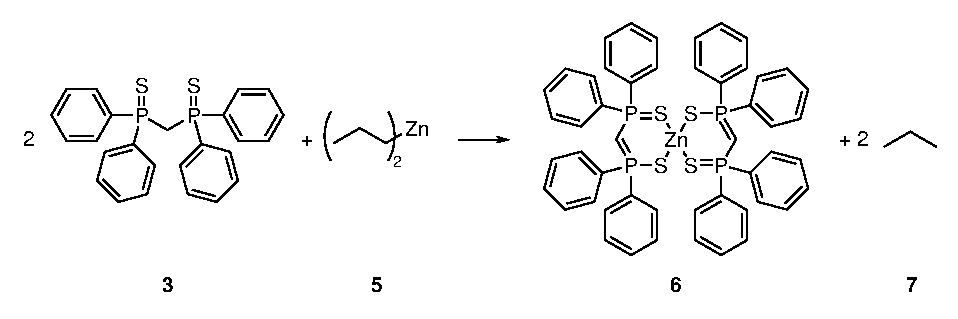
\includegraphics[scale=\ocscale]{Komplex.eps}
    \caption{Eine Synthese f\"ur die Tonne}
    \label{ACFKomplex\suscode}
\end{scheme}
Alternativ geht auch die Feststellung der Breite mit linewidth:
\begin{scheme}[H]
    \centering
    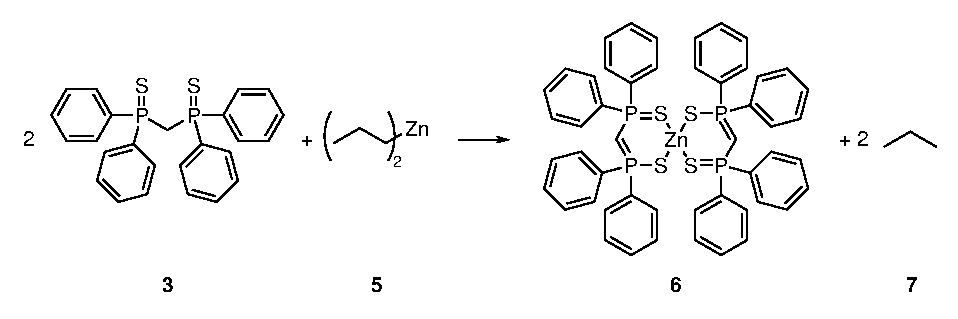
\includegraphics[width=0.85\linewidth]{Komplex.eps}
    \caption{Zweite Synthese f\"ur die Tonne}
\end{scheme}

Zu der Darstellung der OC- L\"osungsk\"astchen dient der Befehl:\\
In der folgenden Teilaufgabe folgt das Einf\"ugen von OC Formeln Bildern und OC K\"astchen. 

\ocanfang
\oc{\textbf{1}}{
\includegraphics[scale=\ocscale]{beta_lacton.eps}}{}
\oc{\textbf{2}}{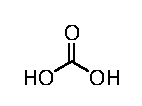
\includegraphics[scale=\ocscale]{H2CO3.eps}}{}
\oc{\textbf{3}}{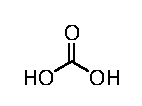
\includegraphics[width=0.5\linewidth]{H2CO3.eps}}{}
\ockasten{112}{4}
\ocende
% \kastenarray
%     [] % Breite (kann weggelassen werden, dann an Inhalt angepasst)
%     {4cm} % H\"ohe
%     [0cm] % Abstand zwischen den K\"astchen (kann weggelassen werden, dann 0cm)
%     [f] %t oder f: t - kein Abstand unter Kasten; f - Abstand unter Kasten (Optional; wenn weggelassen dann =t)
%     {Q,W} % Bezeichnungen
%     {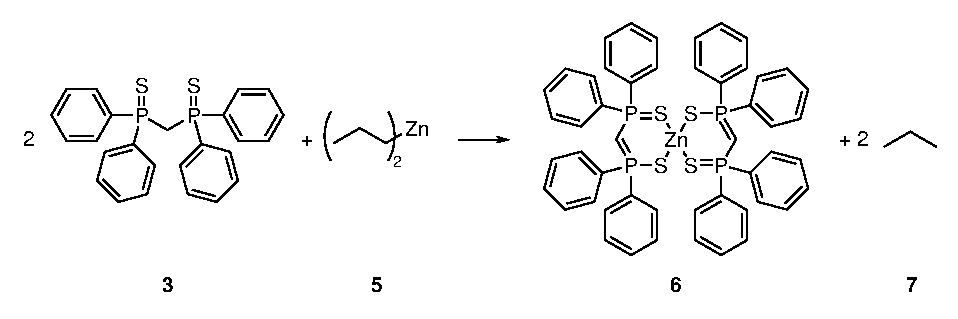
\includegraphics[width=5.5cm]{Komplex.eps},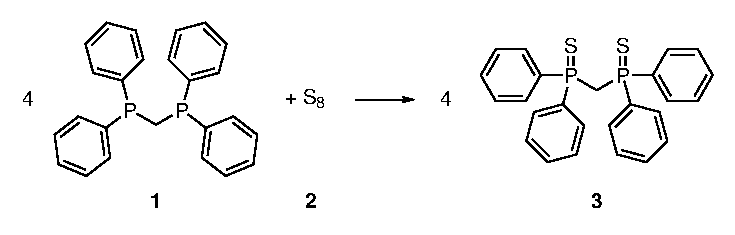
\includegraphics[width=5.5cm]{Ligand.eps}}% Inhalte mit Kommata seperieren
%Man kann diese auch aneinander Reihen: Noch zwei Kastenarrays.
% \kastenarray[7cm]{7cm}{1,2}{Molekuel1,Molekuel2}

\kasten{16cm}{
Reaktion erster Ordnung: \ch{A -> B}\punkte{1}
\begin{align*}
    v(t)&=-\dd{[\ch{A}]}{t}=k\cdot[\ch{A}]\punkte{1}\\
    a(t)&=-\dd[2]{[\ch{A}]}{t}\quad\kommentar{Auch h\"ohere Ableitungen sind m\"oglich.}\\
    \intertext{Mit \textbackslash intertext kann man auch Text in Gleichungen einf\"ugen.}\\
    \frac{\textnormal{d}[\ch{A}]}{[\ch{A}]}&=-k\,\textnormal{d}t\\
    \int_{[\ch{A}]_0}^{[\ch{A}]}\left(\frac{1}{[\ch{A}]}\right)\,\textnormal{d}[\ch{A}]&=\int_0^t -k\,\textnormal{d}t\punkte{1}\\
    &=\ln[\ch{A}]-\ln[\ch{A}]_0=\ln\left(\frac{[\ch{A}]}{[\ch{A}]_0}\right)\\
    \Rightarrow [\ch{A}]&=[\ch{A}]_0\cdot\exp{-k\cdot t}\punkte{1}
\end{align*}
\kommentar{1P f\"ur Rkt. 1. Ordnung, 1P f\"ur Geschwindigkeitsgesetz, 1P f\"ur Integrieren, 1P f\"ur richtiges Ergebni stnhwortnhw oetnho\"owetnh o\"owaen t hoaes nrthaoenrhoa nethae}
}{}
\newpage
\teilaufgabe{\operator{Male} das Mandala aus.\punkte{69}}{Dies wurde nur hinzugef\"ugt, um \textbackslash punkteausgabe zu zeigen.}
\begin{scheme}[H]
    
\includegraphics[width=\linewidth]{mandala.jpg}
\end{scheme}
\punkteausgabe

Hier wurde Punkteausgabe benutzt, da die Aufgabe keine Form benutzt, die die Punkte bereits selbst ausgibt.

\teilaufgabe{\operator{Einige Leute} wollen den SuS bereits einen Text in den Antwortkasten schreiben.}{Um dies flexibel zu erm\"oglichen, kann man \textbackslash selfkasten nutzen.}
\selfkasten{5cm}{
    \vspace{5pt}
    \setstretch{1.3}
    In diesem L\"uckentext werden L\"ucken mittels \opt{0}{\_\_\_\_\_\_\_\_\_\_\_   }\sol{\underline{\textbackslash opt\{0\} und \textbackslash sol}}\opt{2}{\punkte{2}} dargestellt. Um die L\"ucken des Textes zu sehen, kannst du im main.tex \textbackslash solution auf \opt{0}{\_\_}\sol{\underline{0}}\opt{2}{\punkte{1}} setzen.\par
    Hier wird noch die Punktzahl der Teilaufgabe halbiert \punktehalbieren
}

Formeln im Text k\"onnen mit align und labeln erstellt werden, um verlinkt zu werden z.B. Gleichung \ref{G:test-Gl\suscode}:
\begin{align}
    pV &= nRT \label{G:test-Gl\suscode}\\
    % Beim Label wurde der Sch\"ulercode mit eingef\"ugt, um im Serienbrief Probleme zu vermeiden
    a &= b
\end{align}
\begin{equation*}
    Q = I \cdot t
\end{equation*}
In Gleichung ist das ideale Gasgesetz gezeigt\ldots 
Im Text sollten Vorzeichen wie bei $\delta-$/$\delta+$ besser au\ss{}erhalb des Mathemodusses stehen, aber ein richtiges Minuszeichen verwenden: $\delta$+/$\delta$\textminus{}\\
Auch innerhalb eines Kastens sind solche Formelumgebungen m\"oglich. Zudem sind Punkte und Kommentare in aligns m\"oglich:\par
\kasten{5cm}{
\begin{align*}
    y = x^2 \punkte{2}\kommentar{\ Kommentar}
\end{align*}
Dies ist die Antwort. Dies ist Antwortsatz 2.
}{}
Hier kommt mal eine andere Aufz\"ahlung:
\begin{enumerate}[(i)]
    \item Hallo
    \item Tsch\"uss
\end{enumerate}

Ein bisschen Millimeterpapier:\\
\kasten{10cm}{
\begin{center}
    \millipapier{1}{16}{9}
\end{center}
}{}


Zwei Tabellen voller Daten:
\begin{table}[H]
    \caption{Tabelle mit verschiedenen thermodynamischen Daten ausgew\"ahlter Stoffe bei $\SI{298}{\kelvin}$.}
    \label{tab: 2025-10-3_therm. Daten\suscode}
    \centering
    \begin{tabular}{|c|C{1.5cm}|C{1.5cm}|C{1.5cm}|C{1.5cm}|}
    \hline
        & \ch{CH4} & \ch{H2O} & \ch{CO} & \ch{H2}\\\hline
        $\Delta_fH^{\circ}_m$ / $\si{\kilo\joule\per\mole}$ & -74,85 & -241,8 & -110,5 & 0\\\hline
        $S^{\circ}_m$ / $\si{\joule\per\mole\per\kelvin}$ & 186,2 & 188,9 & 198,0 & 130,6\\\hline
        $C_{p, m}$ / $\si{\joule\per\mole\per\kelvin}$ & 35,31 & 33,58 & 29,14 & 28,82\\\hline
    \end{tabular}
\end{table}

\begin{table}[H]
    \caption{Tabelle mit verschiedenen thermodynamischen Daten ausgew\"ahlter Stoffe bei $\SI{298}{\kelvin}$.}
    \label{tab: 2025-10-3_therm. Daten2\suscode}
    \centering
    \begin{tabular}{cC{1.5cm}C{1.5cm}C{1.5cm}C{1.5cm}}
    \toprule
        & \ch{CH4} & \ch{H2O} & \ch{CO} & \ch{H2}\\\midrule
        $\Delta_fH^{\circ}_m$ / $\si{\kilo\joule\per\mole}$ & -74,85 & -241,8 & -110,5 & 0\\
        $S^{\circ}_m$ / $\si{\joule\per\mole\per\kelvin}$ & 186,2 & 188,9 & 198,0 & 130,6\\
        $C_{p, m}$ / $\si{\joule\per\mole\per\kelvin}$ & 35,31 & 33,58 & 29,14 & 28,82\\\bottomrule
    \end{tabular}
\end{table}

\aufgabenende
\end{document}
